
\documentclass[10pt]{beamer}
\usepackage{amsmath}
\usepackage{mathtools}
\usepackage{multimedia}
\usepackage{hyperref}


\usefonttheme{professionalfonts} % using non standard fonts for beamer
\usefonttheme{serif} % default family is serif
%\documentclass[12pt]{beamerthemeSam.sty}
\usepackage{epsf}
%\usepackage{pstricks}
%\usepackage[orientation=portrait,size=A4]{beamerposter}
\geometry{paperwidth=160mm,paperheight=120mm}
%DT favorite definitions
\def\LL{\left\langle}	% left angle bracket
\def\RR{\right\rangle}	% right angle bracket
\def\LP{\left(}		% left parenthesis
\def\RP{\right)}	% right parenthesis
\def\LB{\left\{}	% left curly bracket
\def\RB{\right\}}	% right curly bracket
\def\PAR#1#2{ {{\partial #1}\over{\partial #2}} }
\def\PARTWO#1#2{ {{\partial^2 #1}\over{\partial #2}^2} }
\def\PARTWOMIX#1#2#3{ {{\partial^2 #1}\over{\partial #2 \partial #3}} }

\def\rightpartial{{\overrightarrow\partial}}
\def\leftpartial{{\overleftarrow\partial}}
\def\diffpartial{\buildrel\leftrightarrow\over\partial}

\def\BS{\bigskip}
\def\BC{\begin{center}}
\def\EC{\end{center}}
\def\BN{\begin{enumerate}}
\def\EN{\end{enumerate}}
\def\BI{\begin{itemize}}
\def\EI{\end{itemize}}
\def\BE{\begin{displaymath}}
\def\EE{\end{displaymath}}
\def\BEA{\begin{eqnarray*}}
\def\EEA{\end{eqnarray*}}
\def\BNEA{\begin{eqnarray}}
\def\ENEA{\end{eqnarray}}
\def\EL{\nonumber\\}

\newcommand{\etal}{{\it et al.}}
\newcommand{\gbeta}{6/g^2}
\newcommand{\la}[1]{\label{#1}}
\newcommand{\ie}{{\em i.e.\ }}
\newcommand{\eg}{{\em e.\,g.\ }}
\newcommand{\cf}{cf.\ }
\newcommand{\etc}{etc.\ }
\newcommand{\atantwo}{{\rm atan2}}
\newcommand{\Tr}{{\rm Tr}}
\newcommand{\dt}{\Delta t}
\newcommand{\op}{{\cal O}}
\newcommand{\msbar}{{\overline{\rm MS}}}
\def\chpt{\raise0.4ex\hbox{$\chi$}PT}
\def\schpt{S\raise0.4ex\hbox{$\chi$}PT}
\def\MeV{{\rm Me\!V}}
\def\GeV{{\rm Ge\!V}}

%AB: my color definitions
%\definecolor{mygarnet}{rgb}{0.445,0.184,0.215}
%\definecolor{mygold}{rgb}{0.848,0.848,0.098}
%\definecolor{myg2g}{rgb}{0.647,0.316,0.157}
\definecolor{A}{rgb}{1.0,0.3,0.3}
\definecolor{B}{rgb}{0.0,1.0,0.0}
\definecolor{C}{rgb}{1.0,1.0,0.0}
\definecolor{D}{rgb}{0.5,0.5,1.0}
\definecolor{E}{rgb}{0.7,0.7,0.7}
\definecolor{abtitlecolor}{rgb}{1.0,1.0,1.0}
\definecolor{absecondarycolor}{rgb}{0.0,0.416,0.804}
\definecolor{abprimarycolor}{rgb}{1.0,0.686,0.0}
\definecolor{Red}           {rgb}{1,0.4,0.4}
\definecolor{Yellow}           {rgb}{1,1,0.0}
\definecolor{Grey}          {cmyk}{.7,.7,.7,0}
\definecolor{Blue}          {cmyk}{1,1,0,0}
\definecolor{Green}         {cmyk}{1,0,1,0}
\definecolor{Brown}         {cmyk}{0,0.81,1,0.60}
\definecolor{Silver}        {rgb}{0.95,0.9,1.0}
\definecolor{Sky}           {rgb}{0.07,0.0,0.2}
\definecolor{Darkbrown}     {rgb}{0.4,0.3,0.2}
\definecolor{40Gray}        {rgb}{0.4,0.4,0.5}
\usetheme{Madrid}


\setbeamercolor{normal text}{fg=Silver,bg=Sky}

%AB: redefinition of beamer colors
%\setbeamercolor{palette tertiary}{fg=white,bg=mygarnet}
%\setbeamercolor{palette secondary}{fg=white,bg=myg2g}
%\setbeamercolor{palette primary}{fg=black,bg=mygold}
\setbeamercolor{title}{fg=abtitlecolor}
\setbeamercolor{frametitle}{fg=abtitlecolor}
\setbeamercolor{palette tertiary}{fg=white,bg=Darkbrown}
\setbeamercolor{palette secondary}{fg=white,bg=absecondarycolor}
\setbeamercolor{palette primary}{fg=white,bg=40Gray}
\setbeamercolor{structure}{fg=abtitlecolor}

\setbeamerfont{section in toc}{series=\bfseries}

%AB: remove navigation icons
\beamertemplatenavigationsymbolsempty
\title[Astromechanics: gravity]{
  \textbf {Astromechanics: gravity}}


\author [Astronomy 101]{Astronomy 101\\Syracuse University, Fall 2022\\Walter Freeman}

\date{\today}

\begin{document}



\frame{\titlepage}


\frame{\frametitle{\textbf{Announcements}}
	
\large
	
	\BI
	\item Homework quiz 4 is Tuesday at the end of class Tuesday. Please make sure you have finished your homework so you can ask questions at the beginning of class.
	\item We'll be doing makeup/retake quizzes next Tuesday in addition to during office hours. I'll send out a signup tomorrow morning.
	
	\BS\pause
	
	\item I'll send the survey tomorrow as well. It will have something unusual on it:
	\BI
	\item You'll have an opportunity to suggest questions for the next exam
	\item If I use your question, you'll obviously know the answer
	\item ... and you'll also get five extra credit points for the exam!
	\EI
	\EI
	\BS\BS\pause
	
	Prelabs for next week are available in the Physics Clinic and online.
	
	\BS
	
	Next week's lab and prelab involve an online orbit simulator available on the website.
}

\frame{\frametitle{\textbf{Exam 1 retrospective}}

\begin{columns}
	\column{0.5\textwidth}
	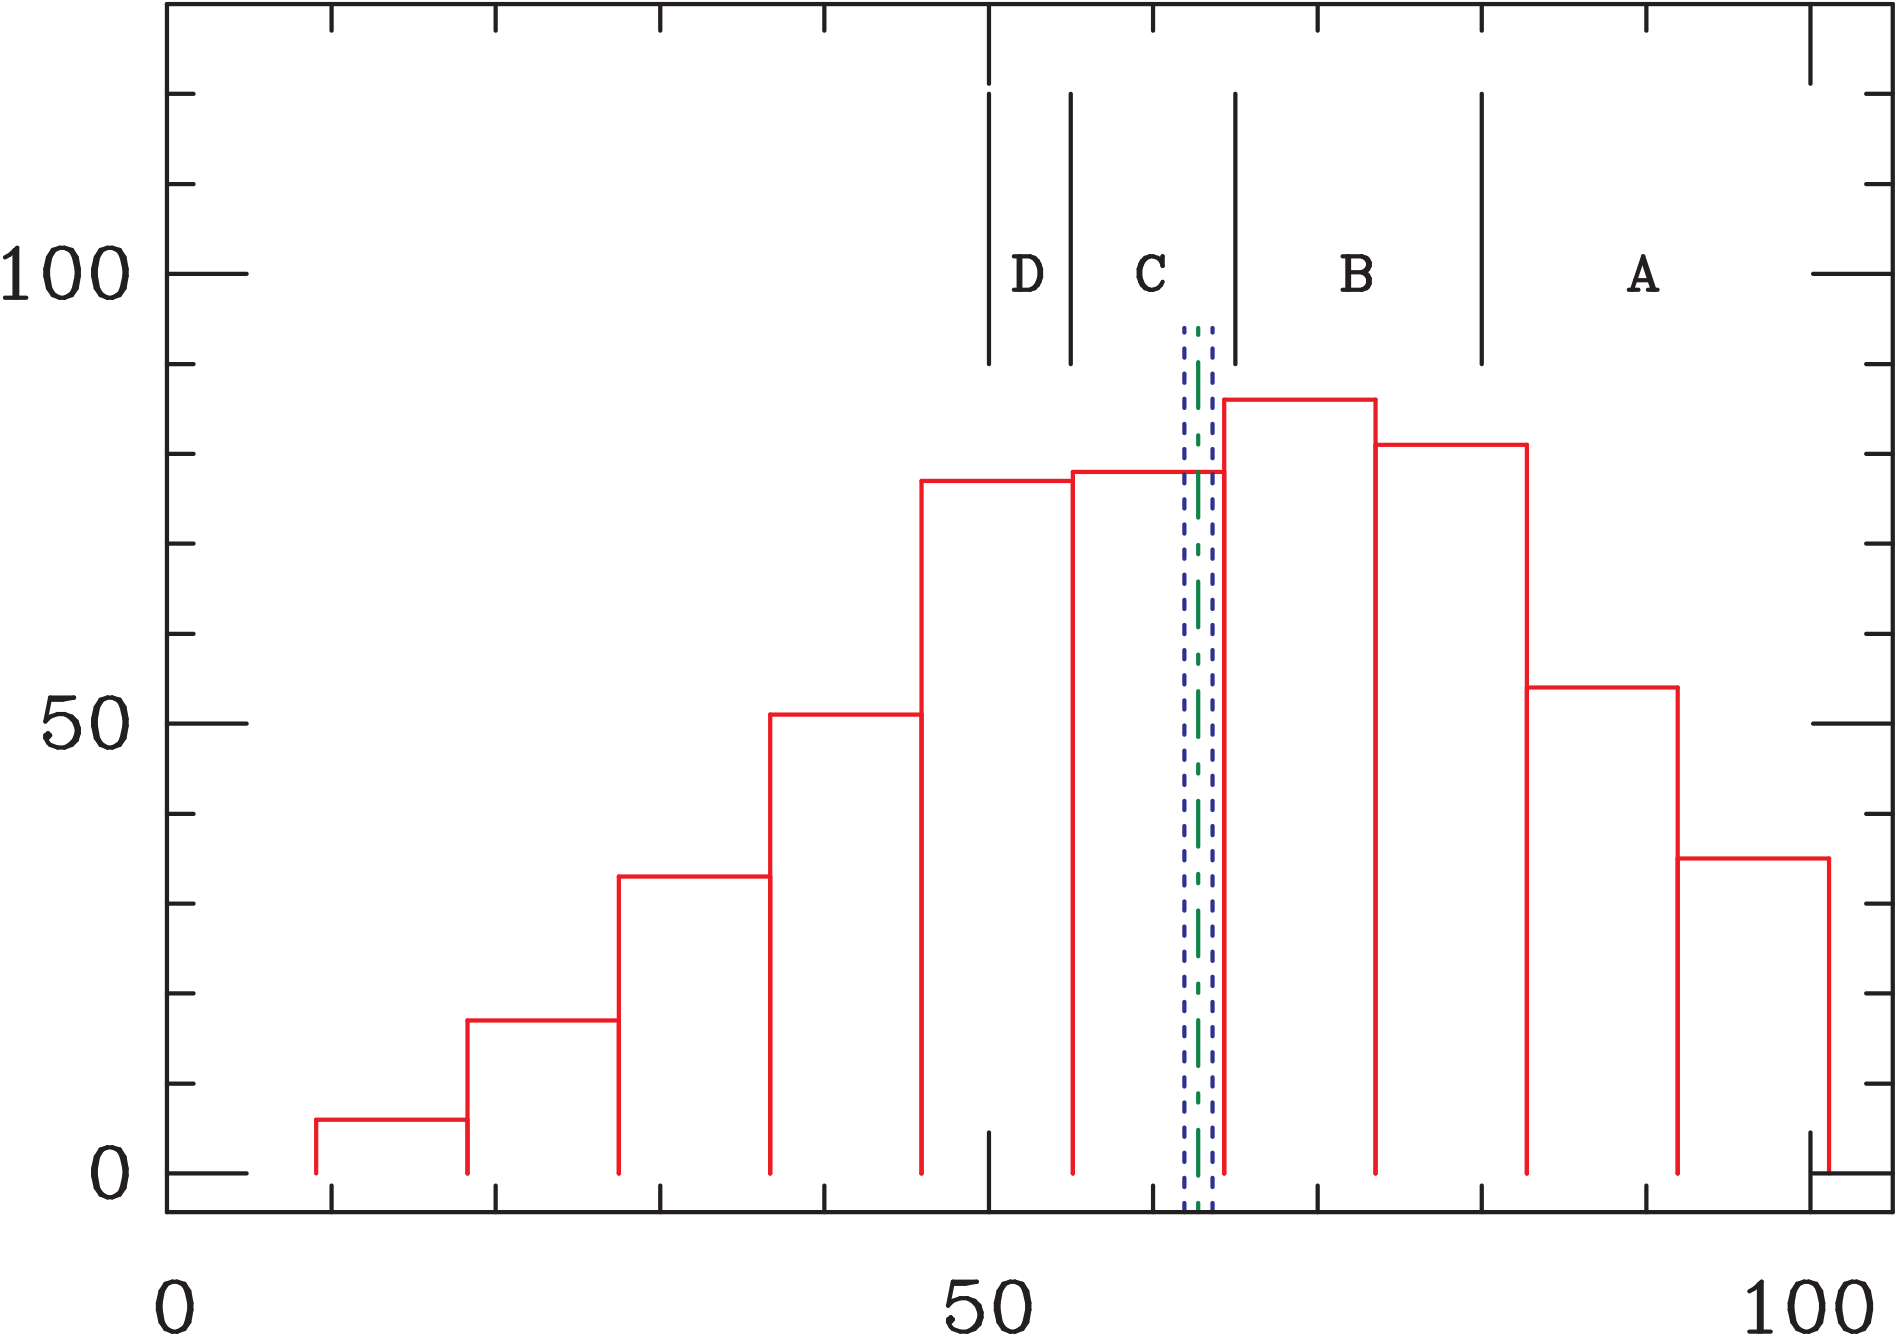
\includegraphics[width=0.9\textwidth]{examhisto.png}
		\BI
	\item Median grade: C+
	\item More A's and B's than D's and F's
	\EI
	
	\column{0.5\textwidth}
	

This is a new format this year (post-pandemic) and people generally did quite well!
	
	\BI
	\item If you did well, congratulations -- you worked hard and it showed.
	\item If you didn't do as well as you had hoped, then we have plenty of semester left!
	\item People's semester grades are generally a good bit higher than their exam average
	\item ... and the first exam is the hardest.
	
	\BS\BS\pause
	
	\item You will have another opportunity to show us that you've mastered this material on the final.
	\item You can {\it absolutely} pass the class regardless of your Exam 1 grade. 
	\item Advice for now: look forward, don't look back too much
	\item Review the solution video for Exam 1 once I make it
	\EI
	
\end{columns}		
	}
		


\frame{\frametitle{\textbf{The law of gravity}}
\Large
Newton showed mathematically what Kepler suspected: that ``there is a force in the Earth that causes the Moon to move''.

\BS
That thing, of course, is gravity.
\BS\BS

Newton discovered:


\bigskip
\bigskip

All objects attract all other objects with a force that is:

\BI
\item{Proportional to the product of their masses}
\item{Inversely proportional to the distance between their centers, squared}
\EI

In symbols:

$$F = \frac{G m_1 m_2}{r^2}$$
}


\frame{
\BC
	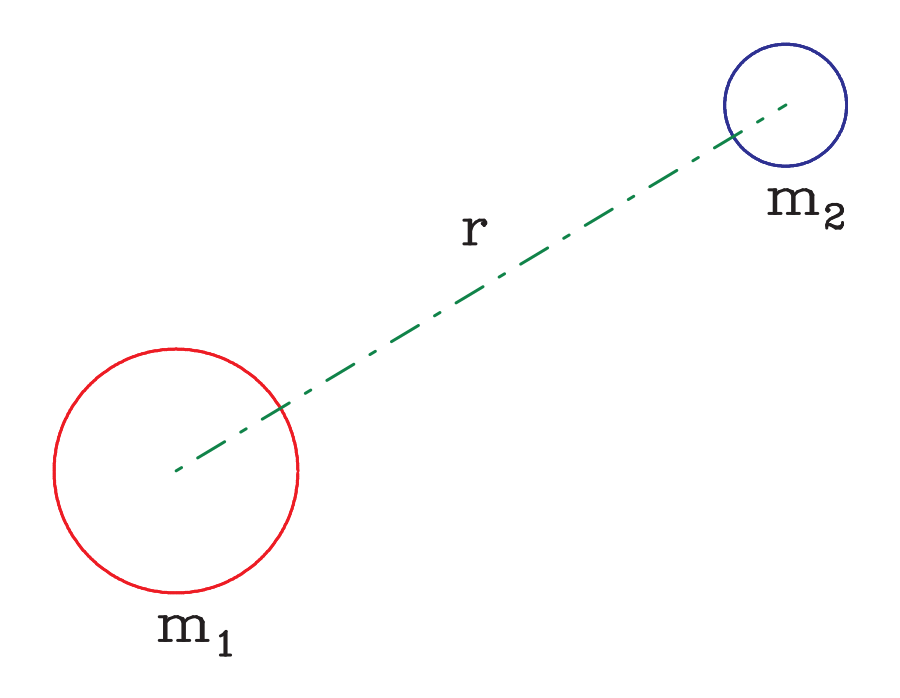
\includegraphics[width=0.65\textwidth]{law-gravity-crop.png}
	
	\Large
	
	\BS
	
	\Large
	
	The gravitational force between these two planets is $$F_g = \frac{G m_1 m_2}{r^2}.$$
\EC	
}

\frame{
	\begin{minipage}{0.5\textwidth}
		\hspace{0.15\textwidth}
			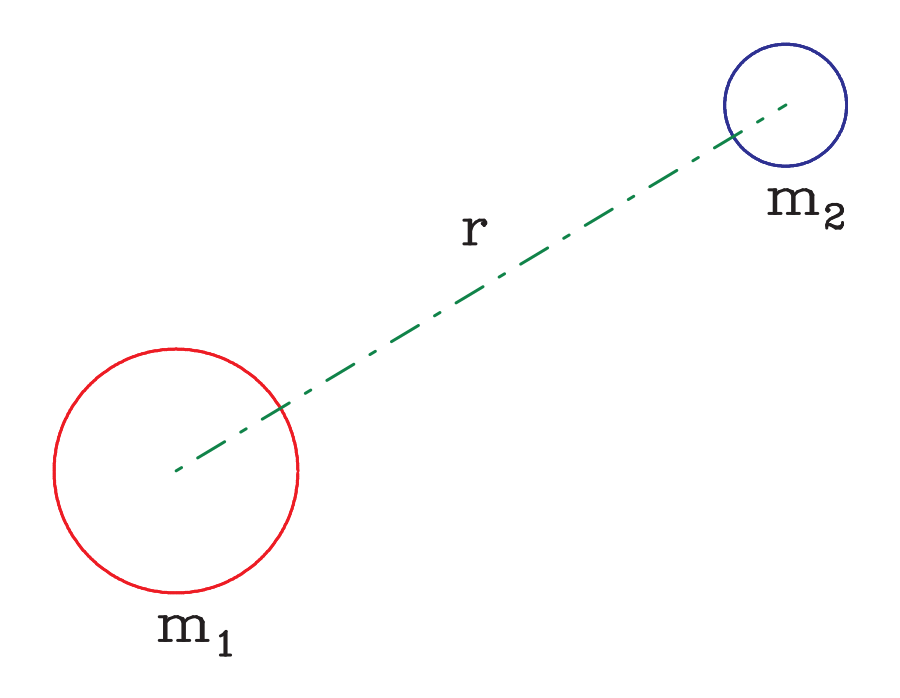
\includegraphics[width=0.7\textwidth]{law-gravity-crop.png}
	\end{minipage}
\begin{minipage}{0.49\textwidth}
	Here's the same diagram again. Suppose $m_1$ is a planet and $m_2$ its moon. As before the force on the moon is
	
	$$F_g = \frac{Gm_1m_2}{r^2}$$
	\end{minipage}

\Large

\BS\BS\BS

Suppose we make the planet twice as massive. How does the gravitational force on the moon change?

\BS\BS

\begin{minipage}{0.59\textwidth}
\color{A}A: It doesn't change

\color{B}B: It becomes twice as strong

\color{C}C: It becomes four times as strong

		\color{D}D: It becomes half as strong

\color{E}E: It becomes one-quarter as strong
\end{minipage}\pause
\begin{minipage}{0.4\textwidth}
	
	$$
	F_g = \frac{G{\color{Red}m_1}m_2}{r^2}
	$$
\end{minipage}
}

\frame{
	\begin{minipage}{0.5\textwidth}
		\hspace{0.15\textwidth}
		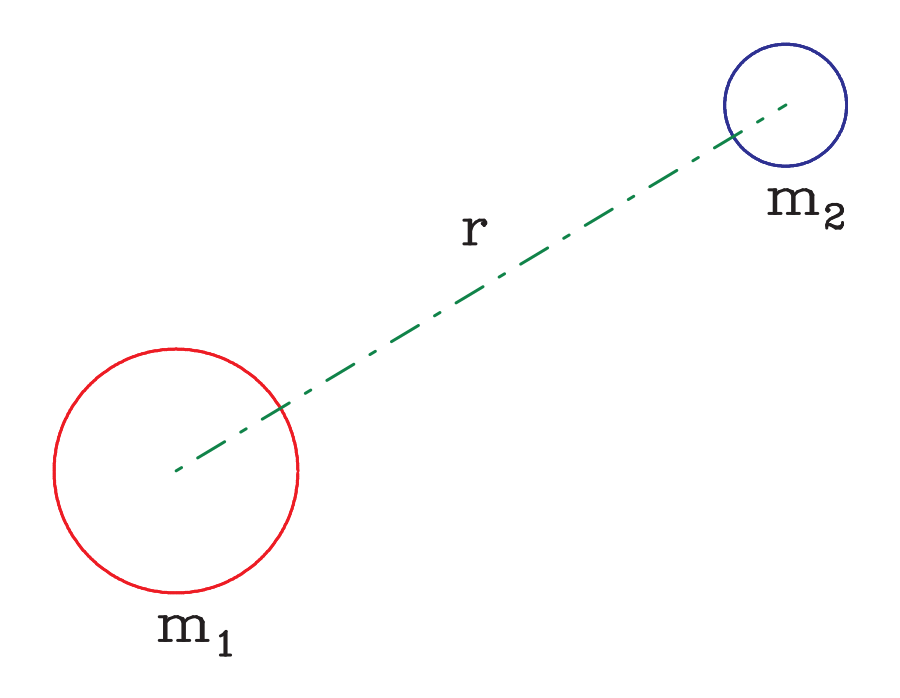
\includegraphics[width=0.7\textwidth]{law-gravity-crop.png}
	\end{minipage}
	\begin{minipage}{0.49\textwidth}
		Here's the same diagram again. Suppose $m_1$ is a planet and $m_2$ its moon. As before the force on the moon is
		
		$$F_g = \frac{Gm_1m_2}{r^2}$$
	\end{minipage}
	
	\Large
	
	\BS\BS\BS
	
	Suppose we make the planet twice as massive. How does the gravitational force on the moon change?
	
	\BS\BS
	
	\begin{minipage}{0.59\textwidth}
		\color{A}A: It doesn't change
		
		\color{B}B: It becomes twice as strong
		
		\color{C}C: It becomes four times as strong
		
			\color{D}D: It becomes half as strong
	
	\color{E}E: It becomes one-quarter as strong
	\end{minipage}
	\begin{minipage}{0.4\textwidth}
		
		$$
		F_g = \frac{G{\color{Red}(2m_1)}m_2}{r^2}
		$$
	\end{minipage}
}

\frame{
	\begin{minipage}{0.5\textwidth}
		\hspace{0.15\textwidth}
		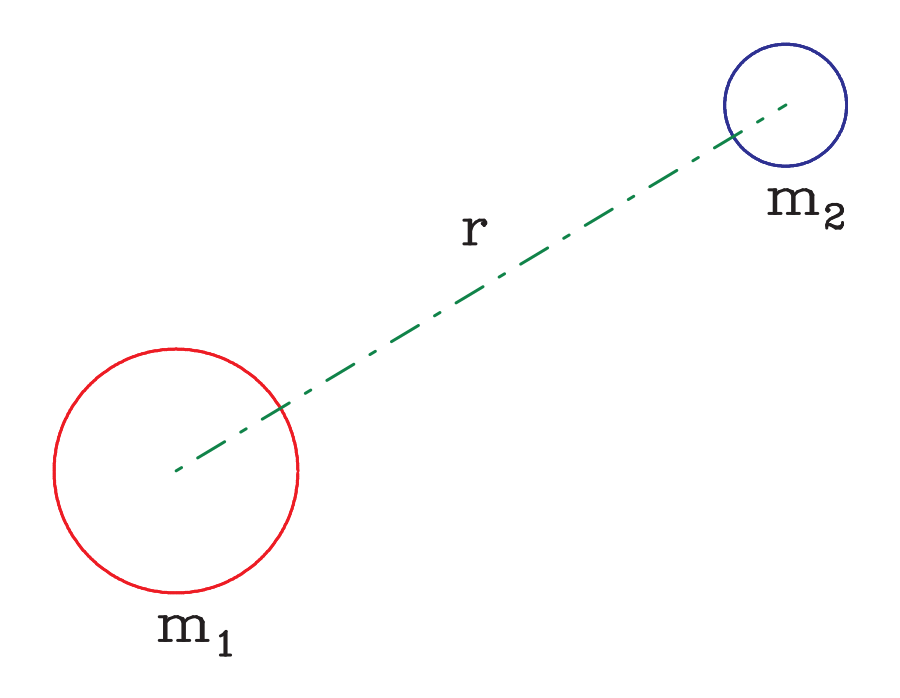
\includegraphics[width=0.7\textwidth]{law-gravity-crop.png}
	\end{minipage}
	\begin{minipage}{0.49\textwidth}
		Here's the same diagram again. Suppose $m_1$ is a planet and $m_2$ its moon. As before the force on the moon is
		
		$$F_g = \frac{Gm_1m_2}{r^2}$$
	\end{minipage}
	
	\Large
	
	\BS\BS\BS
	
	Suppose we make the planet twice as massive. How does the gravitational force on the moon change?
	
	\BS\BS
	
	\begin{minipage}{0.59\textwidth}
		\color{A}A: It doesn't change
		
		\color{B}B: It becomes twice as strong
		
		\color{C}C: It becomes four times as strong
		
		\color{D}D: It becomes half as strong
		
		\color{E}E: It becomes one-quarter as strong
	\end{minipage}
	\begin{minipage}{0.4\textwidth}
		
		$$
		F_g = {\color{Red}2}\frac{G{m_1}m_2}{r^2}
		$$
	\end{minipage}
}

\frame{
	\begin{minipage}{0.5\textwidth}
		\hspace{0.15\textwidth}
		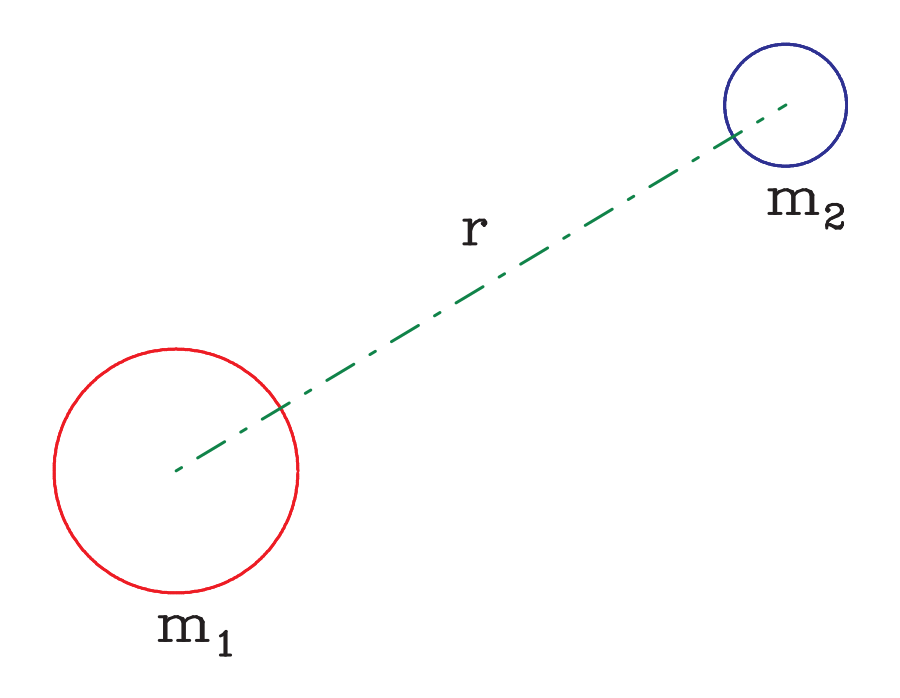
\includegraphics[width=0.7\textwidth]{law-gravity-crop.png}
	\end{minipage}
	\begin{minipage}{0.49\textwidth}
		Again, $m_1$ is a planet and $m_2$ its moon. As before the force on the moon is
		
		$$F_g = \frac{Gm_1m_2}{r^2}$$
	\end{minipage}
	
	\Large
	
	\BS\BS\BS
	
	Suppose we move the moon twice as far away from the planet. How does the gravitational force on the moon change?
	
	\BS\BS
	
	\begin{minipage}{0.59\textwidth}
		\color{A}A: It doesn't change
		
		\color{B}B: It becomes twice as strong
		
		\color{C}C: It becomes four times as strong
		
		\color{D}D: It becomes half as strong
		
		\color{E}E: It becomes one-quarter as strong
	\end{minipage}
\pause
	\begin{minipage}{0.4\textwidth}
		
		$$
		F_g = \frac{Gm_1m_2}{r^2}
		$$
	\end{minipage}
}

\frame{
	\begin{minipage}{0.5\textwidth}
		\hspace{0.15\textwidth}
		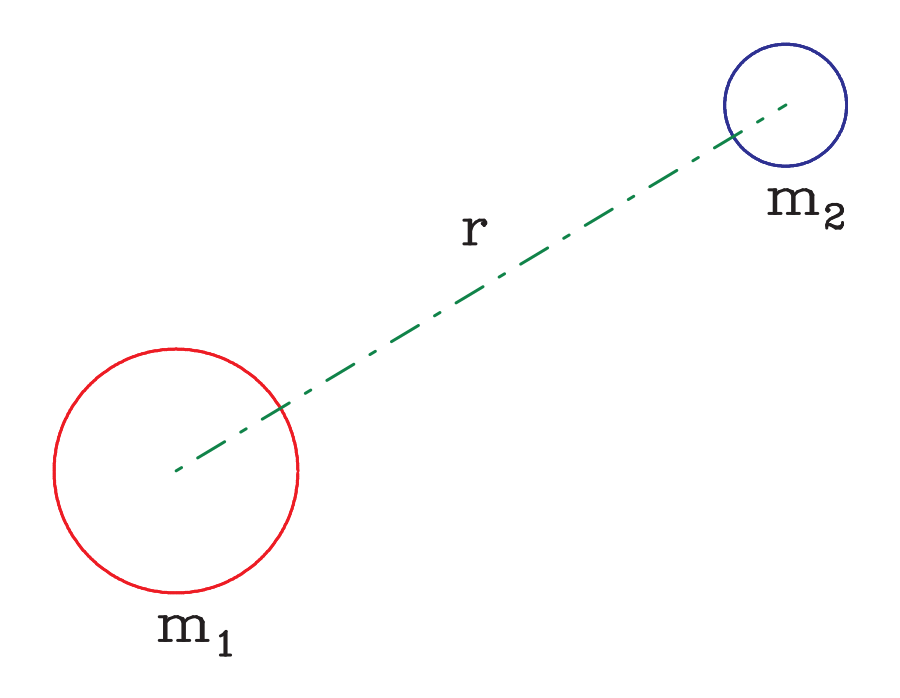
\includegraphics[width=0.7\textwidth]{law-gravity-crop.png}
	\end{minipage}
	\begin{minipage}{0.49\textwidth}
		Again, $m_1$ is a planet and $m_2$ its moon. As before the force on the moon is
		
		$$F_g = \frac{Gm_1{m_2}}{r^2}$$
	\end{minipage}
	
	\Large
	
	\BS\BS\BS
	
	Suppose we move the moon twice as far away from the planet. How does the gravitational force on the moon change?
	
	\BS\BS
	
	\begin{minipage}{0.59\textwidth}
		\color{A}A: It doesn't change
		
		\color{B}B: It becomes twice as strong
		
		\color{C}C: It becomes four times as strong
		
		\color{D}D: It becomes half as strong
		
		\color{E}E: It becomes one-quarter as strong
	\end{minipage}
	\begin{minipage}{0.4\textwidth}
		
		$$
		F_g = \frac{Gm_1{m_2}}{{\color{B}(2r)}^2}
		$$
	\end{minipage}
}

\frame{
	\begin{minipage}{0.5\textwidth}
		\hspace{0.15\textwidth}
		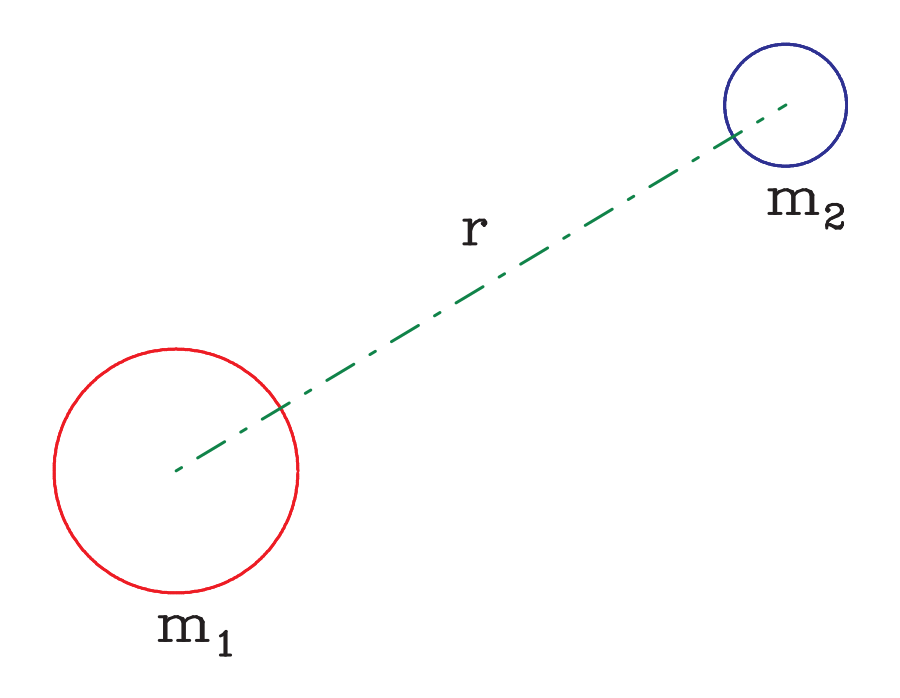
\includegraphics[width=0.7\textwidth]{law-gravity-crop.png}
	\end{minipage}
	\begin{minipage}{0.49\textwidth}
		Here's the same diagram again. Suppose $m_1$ is a planet and $m_2$ its moon. As before the force on the moon is
		
		$$F_g = \frac{Gm_1m_2}{r^2}$$
	\end{minipage}
	
	\Large
	
	\BS\BS\BS
	

Suppose we move the moon twice as far away from the planet. How does the gravitational force on the moon change?
	
	\BS\BS
	
	\begin{minipage}{0.59\textwidth}
		\color{A}A: It doesn't change
		
		\color{B}B: It becomes twice as strong
		
		\color{C}C: It becomes four times as strong
		
		\color{D}D: It becomes half as strong
		
		\color{E}E: It becomes one-quarter as strong
	\end{minipage}
	\begin{minipage}{0.4\textwidth}
		
		$$
			F_g = \frac{Gm_1{m_2}}{{\color{B}4r^2}}
		$$
	\end{minipage}
}

\frame{
	\begin{minipage}{0.5\textwidth}
		\hspace{0.15\textwidth}
		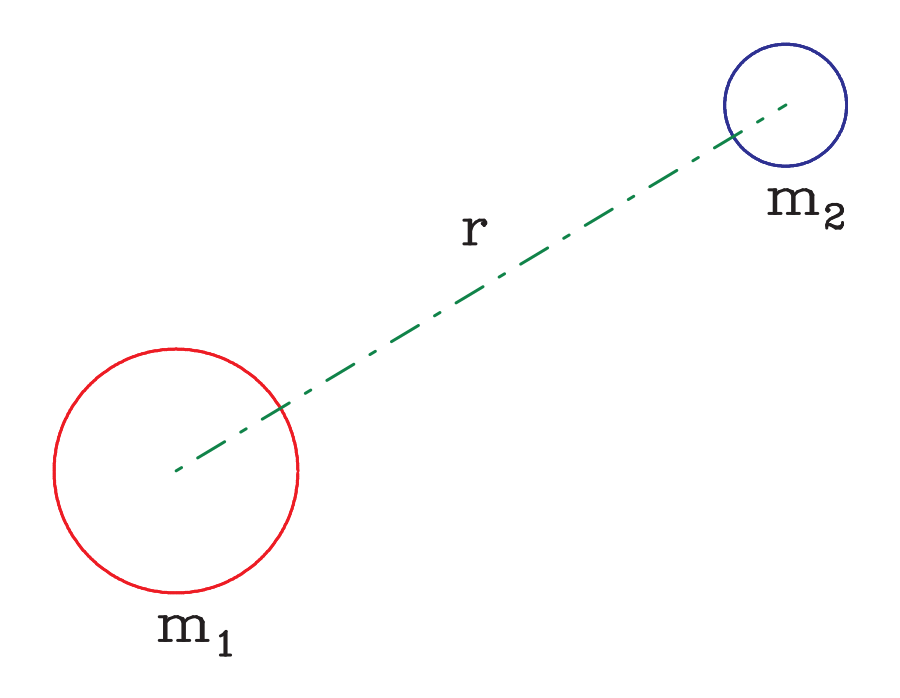
\includegraphics[width=0.7\textwidth]{law-gravity-crop.png}
	\end{minipage}
	\begin{minipage}{0.49\textwidth}
		Here's the same diagram again. Suppose $m_1$ is a planet and $m_2$ its moon. As before the force on the moon is
		
		$$F_g = \frac{Gm_1m_2}{r^2}$$
	\end{minipage}
	
	\Large
	
	\BS\BS\BS
	
	
	Suppose we move the moon twice as far away from the planet. How does the gravitational force on the moon change?
	
	\BS\BS
	
	\begin{minipage}{0.59\textwidth}
		\color{A}A: It doesn't change
		
		\color{B}B: It becomes twice as strong
		
		\color{C}C: It becomes four times as strong
		
		\color{D}D: It becomes half as strong
		
		\color{E}E: It becomes one-quarter as strong
	\end{minipage}
	\begin{minipage}{0.4\textwidth}
		
		$$
		F_g = {\color{B}\frac{1}{4}}\frac{Gm_1{m_2}}{r^2}
		$$
	\end{minipage}
}



\frame{
	\begin{minipage}{0.5\textwidth}
		\hspace{0.15\textwidth}
		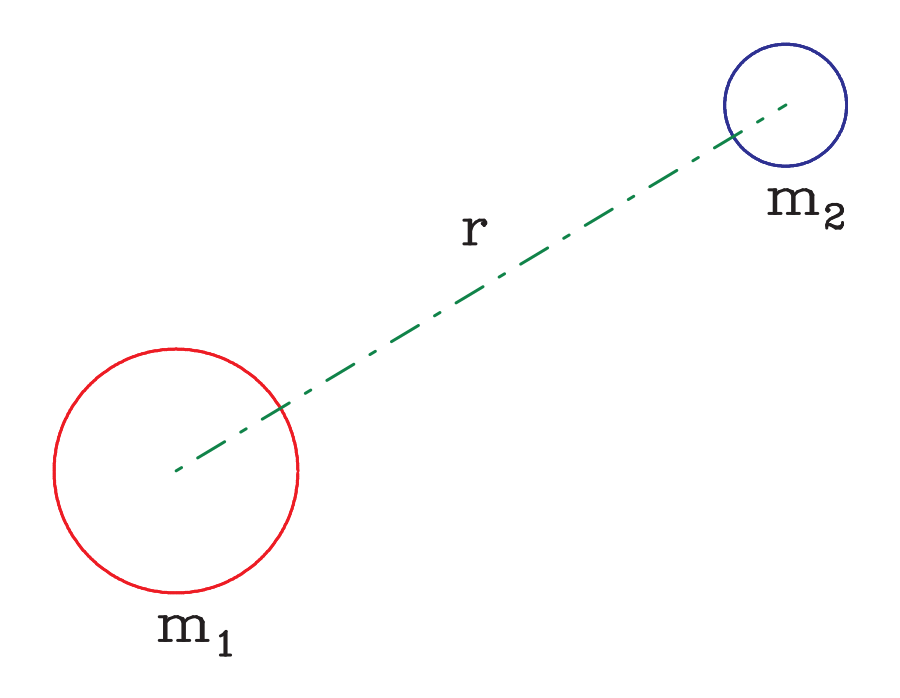
\includegraphics[width=0.7\textwidth]{law-gravity-crop.png}
	\end{minipage}
	\begin{minipage}{0.49\textwidth}
		Here's the same diagram again. Suppose $m_1$ is a planet and $m_2$ its moon, and $m_1$ is twice as big as $m_2$. As before the force that the planet applies to the moon is
		
		$$F_g = \frac{Gm_1m_2}{r^2}$$
	\end{minipage}
	
	
	\BS\BS\BS
	
	How does the force that the moon applies on the planet compare to the force the planet applies to the moon?
	
	\BS\BS
	
	\begin{minipage}{0.75\textwidth}
		
		\normalsize
		
		\color{A}A: The force on the planet is twice as large as the force on the moon
		
		\color{B}B: The force on the planet is four times as large as the force on the moon
		
		\color{C}C: The force on the planet is half as large as the force on the moon
		
		\color{D}D:The force on the planet is one-quarter as large as the force on the moon
		
		\color{E}E: Both planets pull on one another with the same force.
	\end{minipage}
\pause
	\begin{minipage}{0.24\textwidth}
		\large
		$$
		F_g = \frac{G{\color{A} m_1}\color{B} m_2}{r^2}
		$$
	\end{minipage}
}





\frame{\frametitle{\textbf{The law of gravity}}
\Large

All objects attract all other objects with a force that is:

\BI
\item{Proportional to the product of their masses}
\item{Inversely proportional to the distance between them squared}
\EI

In symbols:

$$F = \frac{G m_1 m_2}{r^2}$$

\BC
\color{Red}
Notice I didn't say which mass was which. It doesn't matter!
\EC

}

\frame{
\Large
Suppose two asteroids are floating out in space, 20 miles apart. Asteroid A is twice as massive as asteroid B,
and the force of A's gravity on B is ten tons.

\bigskip

Suppose I now move the two asteroids closer, so they're only 10 miles apart. What will the force of A's gravity on B be now?

\huge

\bigskip

\color{A}A: 5 tons\\
\color{B}B: 10 tons\\
\color{C}C: 20 tons\\
\color{D}D: 40 tons
}

\frame{

\BC

\Large

The distance is measured between the {\it centers} of the objects.

\BS

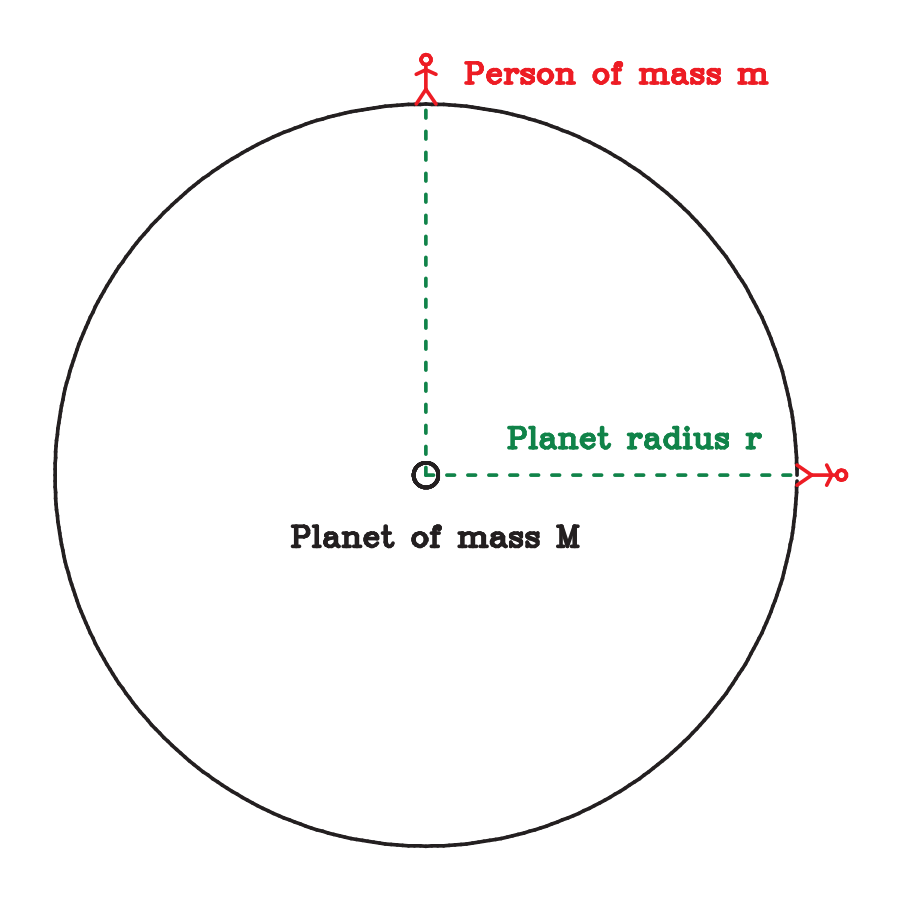
\includegraphics[width=0.5\textwidth]{planet-grav.png}

	\BS

This lets you calculate the force of a planet's gravity on people on its surface!

\BS

\EC
}
\frame{
	
	\BC
	
	\Large
	
	Earth has a radius of about 6,000 km. If we move this person 6,000~km away from Earth's surface, how does the strength of Earth's gravity change?
	
	\BS
	
	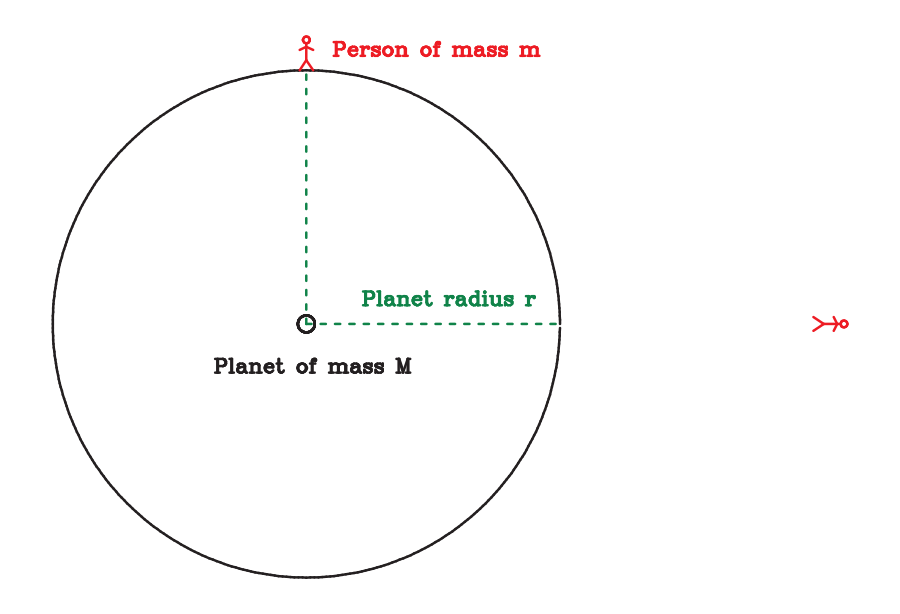
\includegraphics[width=0.7\textwidth]{planet-grav-2.png}
	
	\BS
		
	\EC
}

\frame{
\huge
\color{A}A: It stays the same\\
\color{B}B: It becomes twice as strong\\
\color{C}C: It becomes half as strong\\
\color{D}D: It becomes one-quarter as strong\\
\color{E}E: There's no gravity in space, so it goes away totally\\
}

\frame{\frametitle{\textbf{The ball and the feather}}
	\Large
	We still haven't figured out why this happens: \url {https://www.youtube.com/watch?v=Oo8TaPVsn9Y}
	
	\BS\BS\pause
	
	So far we have talked only about the {\it force} of gravity. 
	
	\BS\BS\pause
	
	The missing piece: {\bf \color{B} how do forces make things move?}
}


\frame{\frametitle{\textbf{Newton's biggest idea}}
	
	\Huge
	\BC
	
	``Forces cause objects to accelerate''
	
	\bigskip
	\bigskip
	\bigskip
	
	$F=ma$
	
	\bigskip
	\bigskip
	\bigskip
	
	$F/m = a$
	
	\bigskip
	\bigskip
	\bigskip
	
	\Large
	
	``The strength of a force, divided by the mass of the thing it acts on, gives that thing's acceleration''
	\EC
}

\frame{\frametitle{\textbf{Newton's biggest idea}}
	
	\Huge
	\BC
	
	Let's apply this to the hammer and the feather and see what happens.
	
	\large
	\BS\BS
	(on document camera)
	
	
	\EC
}


\frame{\frametitle{\textbf{Newton's biggest idea}}
	
\Large

Surprising result: this means that {\it all objects}, regardless of their mass, move in response to 
gravity in the same way!


}

\end{document}
